\documentclass[a4paper,11pt]{article}
\usepackage[italian]{babel}
\usepackage[T1]{fontenc}
\usepackage[utf8]{inputenc}
\usepackage{amsmath}
\usepackage{amsthm}
\usepackage[a4paper,top=1.5cm,bottom=2cm,left=1.5cm,right=1.5cm]{geometry}
\usepackage{amsfonts}
\usepackage{color}
\usepackage{bbm}
\usepackage{datetime}
\usepackage[colorlinks=true]{hyperref}
\usepackage{graphicx}
\usepackage{verbatim}
\usepackage{titlepic}
%\usepackage{physics}
\usepackage{subfigure}
\usepackage{float}

\newcommand{\abs}[1]{\lvert#1\rvert}

\begin{document}

\title{\sc Homework 3}
\author{\sc Alice Schirinà}
\maketitle

\noindent Consideriamo un sistema di molecole monoatomiche che interagiscono tramite il potenziale 
\begin{equation*}
U(r) = A \frac{\sigma e^{-r/\sigma}}{r}
\end{equation*}
quando $ r <r_c $ e $U(r) = 0$ per $ r >r_c $. Scegliamo il lato della scatola cubica $ L/\sigma $ in maniera tale che sia $\rho \sigma^3=0.5$ e utilizziamo unità ridotte, cioè
\begin{table}[H]
	\centering
	\begin{tabular}{l} 
		\hline
		 $Unit\grave{a}\ ridotte$ \\
		\hline
		$r^* = r/\sigma$	\\
		$t^* = t/\sigma \sqrt{A/m}$	\\
		$v^* = v\sqrt{m/A}$	\\
		$E^* = E/A$	\\
		$p^* = p \sigma^3/A$	\\
		$T^* = k_B T/A$	\\\hline
	\end{tabular}
\end{table}
\medskip
\noindent \section*{Configurazione iniziale}
Generiamo una configurazione in cui le molecole sono distribuite casualmente nella scatola di lato $ L/\sigma $ e con velocità anch'esse casuali per cui usiamo il comando $RNG(-0.5,0.5)$. In particolare, vogliamo che sia $\sum v^* = 0$. In generale, questo non accade per cui definiamo la quantità
\begin{equation*}
P^* = \sum_{i=0}^N v_i^*
\end{equation*}
e ridefiniamo velocità ed energia cinetica come segue
\begin{eqnarray}
{v_i^*}' &=& v_i^* - \frac{P^*}{N}\\
K^* &=& \sum_i \frac{1}{2} ({v_i^*}')^2\\
\end{eqnarray}
e infine scaliamo le velocità
\begin{equation*}
\hat{v}_i^* = \alpha {v_i^*}'
\end{equation*}
dove 
\begin{equation*}
\alpha = \sqrt{\frac{0.8N}{K^*}}
\end{equation*}
In questo modo otteniamo particelle disposte casualmente nella scatola con velocità tali che la somma totale sia nulla e con energia cinetica per particella $K^* = 0.8$.\\
Con questa configurazione eseguiamo una simulazione utilizzando lo schema di Verlet per le velocità con passo temporale $\Delta t^* = 0.002$ e fermandoci a $t^* = 1$. Infine, scaliamo ancora una volta le velocità in maniera tale che $K^*/N = 1$. Questa è la nostra configurazione iniziale.
\\
\noindent Partendo dalla stessa configurazione eseguiamo sei simulazioni  ciascuna delle quali con passo temporale diverso
\begin{table}[H]
	\centering
	\begin{tabular}{cl} 
		\hline
		$run$	&	$\Delta t$ \\
		\hline
		$1$	&	$0.001$\\
		$2$	&	$0.003$	\\
		$3$	&	$0.009$	\\
		$4$	&	$0.027$	\\
		$5$	&	$0.081$	\\
		$6$	&	$0.243$	\\\hline
	\end{tabular}
\end{table}
\medskip
\noindent e arrestandoci a $t^* = 25$. Dopo ogni iterazione calcoliamo l'energia potenziale $U(t)$, la pressione istantanea $P(t)$, l'energia totale $E(t)=U(t)+K(t)$ e, infine, la temperatura istantanea $T(t)=2K(t)/3N$, tutte in unità ridotte. Inoltre, a ogni passo Verlet è necessaria anche la forza. Per quest'ultima e per le altre osservabili usiamo le seguenti espressioni:
\begin{eqnarray}
U(r) & = & \frac{e^{-r}}{r}\\
P(r) & = & \frac{NT}{L^{3}} - \frac{e^{-r}}{3L^{3}}\left(\frac{1}{r} + 1\right)\\
K(t) & = & \frac{1}{2}v^2(t)\\
F_{x,i}(r) & = & \frac{x_i}{r^2} \left(1+\frac{1}{r}\right)
\end{eqnarray}
le componenti $y$ e $z$ della forza si calcolano analogamente. Per semplicità di scrittura abbiamo omesso i simboli $^*$ ma ricordiamo ancora una volta che le osservabili in esame sono espresse in unità ridotte. \\Vogliamo ora mostrare gli andamenti dell'energia cinetica per molecola nelle varie simulazioni per trovare quelle stabili.
%grafici
\begin{figure}[H]
	\centering 
	%\subfigure[{Run $1$, $\Delta t^* = 0.001$}]%\label{fig:libraryvoid}
	{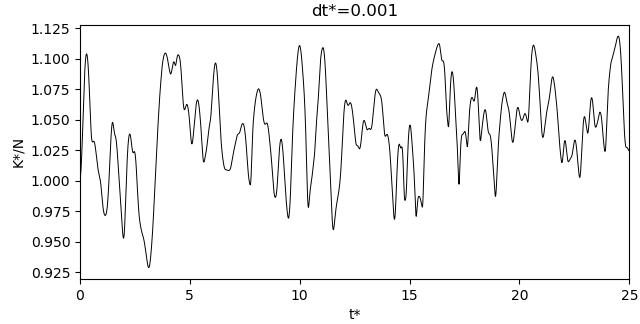
\includegraphics[width=0.65\linewidth]{runstabili/K0001}}\\
	%\subfigure[{Run $2$, $\Delta t^* = 0.003$}]%\label{fig:board}
	{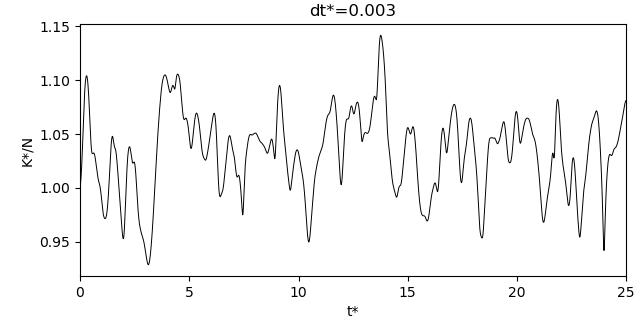
\includegraphics[width=0.65\linewidth]{runstabili/K0003}}\\
\end{figure}
\begin{figure}[H]
	\centering 
	%\subfigure[{Run $3$, $\Delta t^* = 0.009$}]%\label{fig:libraryvoid}
	{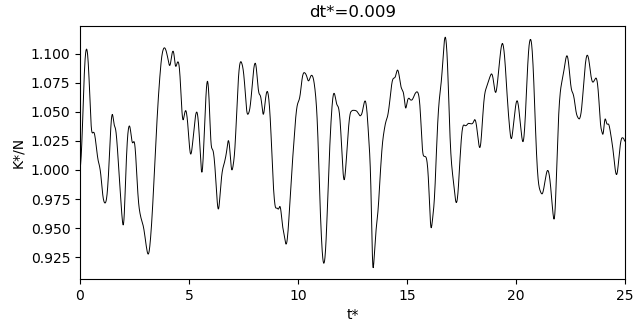
\includegraphics[width=0.65\linewidth]{runstabili/K0009}}\\
	%\subfigure[{Run $4$, $\Delta t^* = 0.027$}]%\label{fig:board}
	{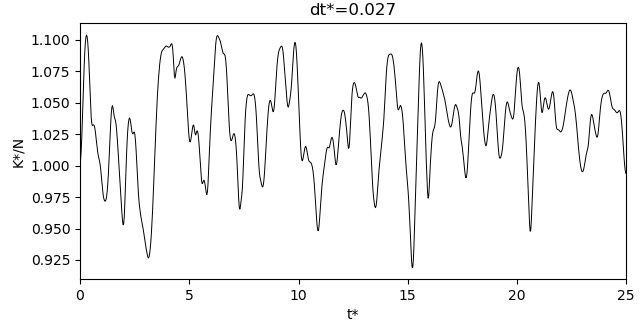
\includegraphics[width=0.65\linewidth]{runstabili/K0027}}\\
\end{figure}
\begin{figure}[H]
	\centering 
	%\subfigure[{Run $5$, $\Delta t^* = 0.081$}]%\label{fig:libraryvoid}
	{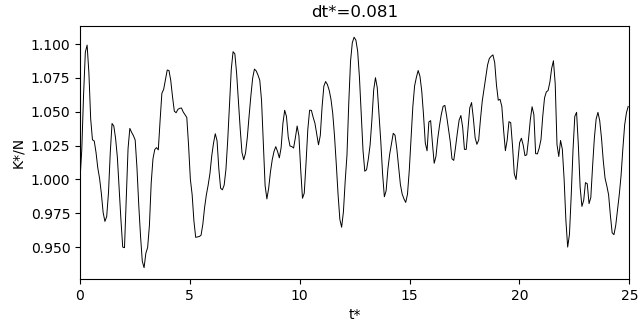
\includegraphics[width=0.65\linewidth]{runstabili/K0081}}\\
	%\subfigure[{Run $6$, $\Delta t^* = 0.243$}]%\label{fig:board}
	{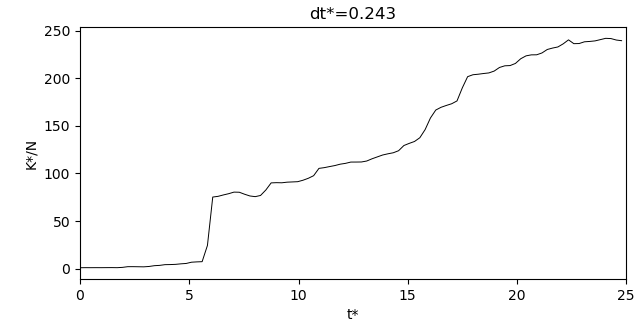
\includegraphics[width=0.65\linewidth]{runstabili/K0243}}\\
	\caption{Andamento energia cinetica per molecola}
\end{figure}
\noindent Come possiamo osservare dal grafico, l'energia nella simulazione con $\Delta t^* = 0.243$ risulta essere instabile per cui eseguiamo la nostra analisi su tutte le simulazioni eccetto questa.

\section*{Divergenza della traiettoria}
Osserviamo ora l'effetto del crescere di $\Delta t^*$ sulle traiettorie delle osservabili. Riportiamo di seguito $E^{(i)}-E^{(1)}$, $P^{(i)}-P^{(1)}$ e $T^{(i)}-T^{(1)}$ dove $i=2,3,4,5$ indica la \textit{run}.
\begin{figure}[H]
	\centering 
	\subfigure[{Run $1$, $\Delta t^* = 0.001$}]%\label{fig:libraryvoid}
	{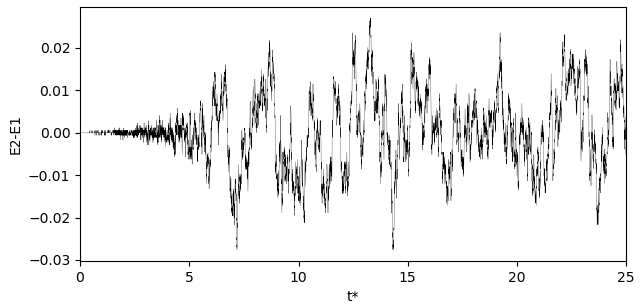
\includegraphics[width=0.48\linewidth]{divergenzaTraiettorie/differenzaEnergia0003}}
	\subfigure[{Run $2$, $\Delta t^* = 0.003$}]%\label{fig:board}
	{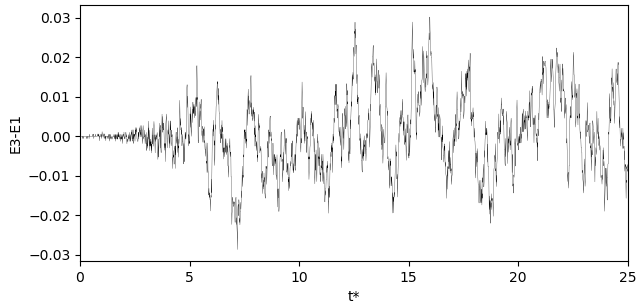
\includegraphics[width=0.48\linewidth]{divergenzaTraiettorie/differenzaEnergia0009}}
	\subfigure[{Run $3$, $\Delta t^* = 0.009$}]%\label{fig:libraryvoid}
	{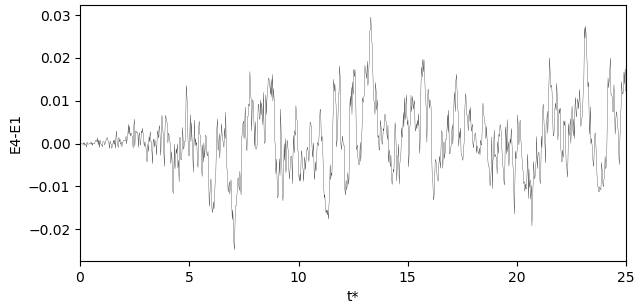
\includegraphics[width=0.48\linewidth]{divergenzaTraiettorie/differenzaEnergia0027}}
	\subfigure[{Run $4$, $\Delta t^* = 0.027$}]%\label{fig:board}
	{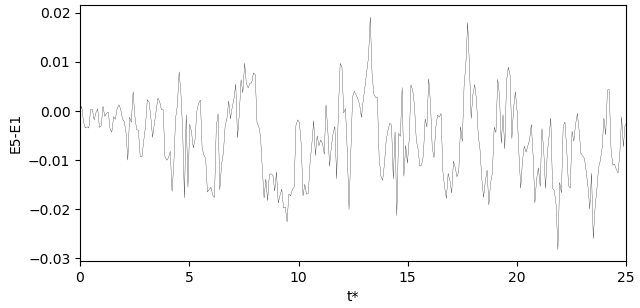
\includegraphics[width=0.48\linewidth]{divergenzaTraiettorie/differenzaEnergia0081}}
	\caption{Divergenza delle traiettorie per l'energia totale}
\end{figure}
\begin{figure}[H]
	\centering 
	\subfigure[{Run $1$, $\Delta t^* = 0.001$}]%\label{fig:libraryvoid}
	{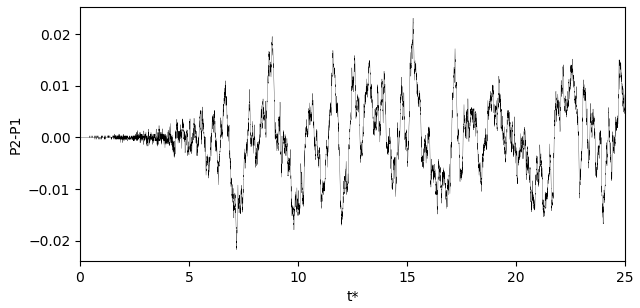
\includegraphics[width=0.48\linewidth]{divergenzaTraiettorie/differenzaPressione0003}}
	\subfigure[{Run $2$, $\Delta t^* = 0.003$}]%\label{fig:board}
	{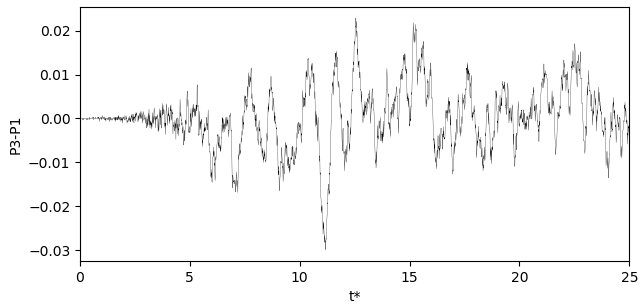
\includegraphics[width=0.48\linewidth]{divergenzaTraiettorie/differenzaPressione0009}}
	\subfigure[{Run $3$, $\Delta t^* = 0.009$}]%\label{fig:libraryvoid}
	{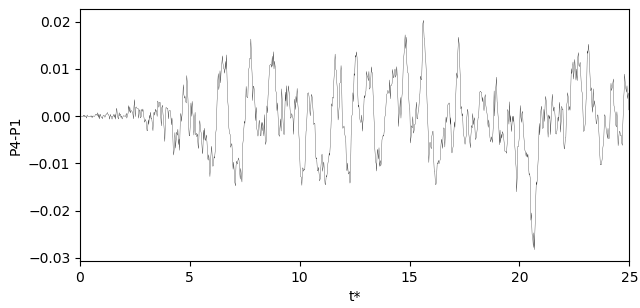
\includegraphics[width=0.48\linewidth]{divergenzaTraiettorie/differenzaPressione0027}}
	\subfigure[{Run $4$, $\Delta t^* = 0.027$}]%\label{fig:board}
	{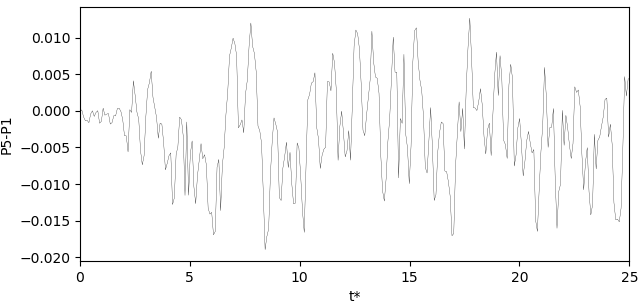
\includegraphics[width=0.48\linewidth]{divergenzaTraiettorie/differenzaPressione0081}}
	\caption{Divergenza delle traiettorie per la pressione}
\end{figure}
\begin{figure}[H]
	\centering 
	\subfigure[{Run $1$, $\Delta t^* = 0.001$}]%\label{fig:libraryvoid}
	{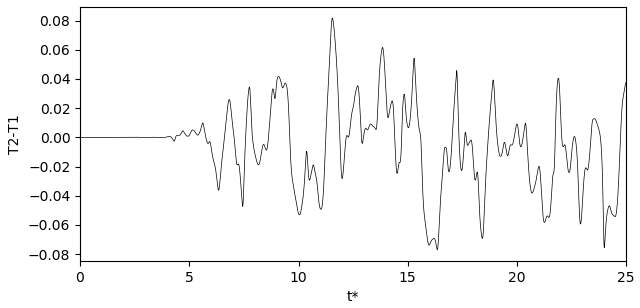
\includegraphics[width=0.48\linewidth]{divergenzaTraiettorie/differenzatemperatura0003}}
	\subfigure[{Run $2$, $\Delta t^* = 0.003$}]%\label{fig:board}
	{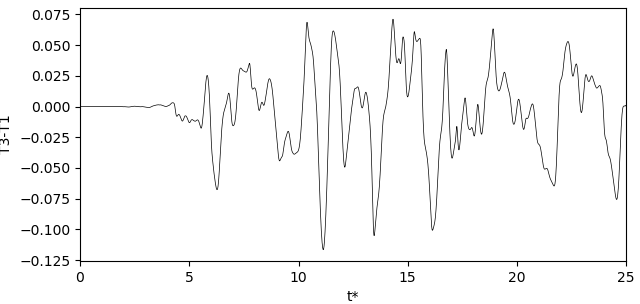
\includegraphics[width=0.48\linewidth]{divergenzaTraiettorie/differenzatemperatura0009}}
	\subfigure[{Run $3$, $\Delta t^* = 0.009$}]%\label{fig:libraryvoid}
	{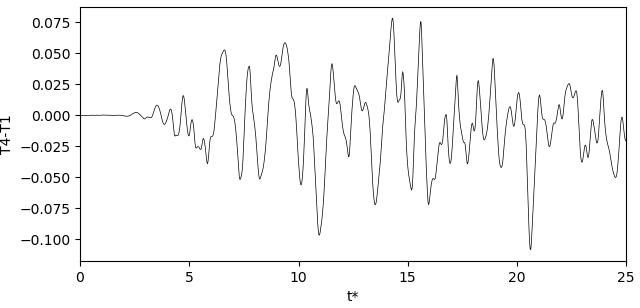
\includegraphics[width=0.48\linewidth]{divergenzaTraiettorie/differenzatemperatura0027}}
	\subfigure[{Run $4$, $\Delta t^* = 0.027$}]%\label{fig:board}
	{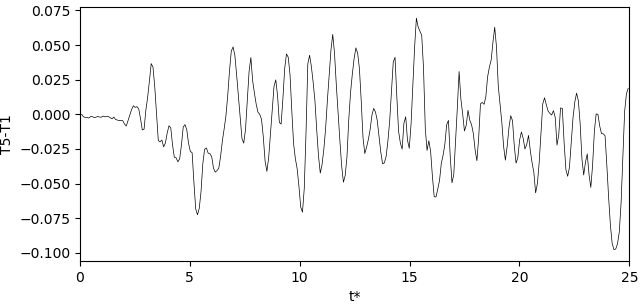
\includegraphics[width=0.48\linewidth]{divergenzaTraiettorie/differenzatemperatura0081}}
	\caption{Divergenza delle traiettorie per la temperatura}
\end{figure}
\newpage
\section*{Conservazione dell'energia}
Osserviamo adesso la conservazione dell'energia riportando i grafici dell'energia totale per le diverse simulazioni.
\begin{figure}[H]
	\centering 
	\subfigure[{Run $1$, $\Delta t^* = 0.001$}]%\label{fig:libraryvoid}
	{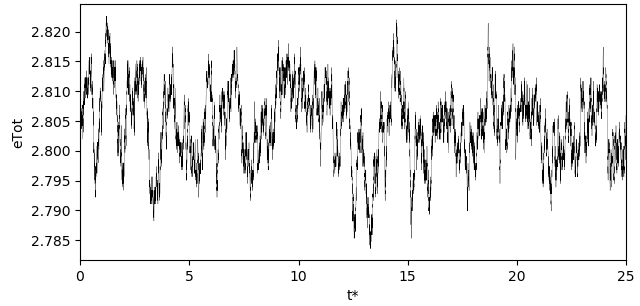
\includegraphics[width=0.7\linewidth]{conservazioneEnergia/eTot0001}}
	\subfigure[{Run $2$, $\Delta t^* = 0.003$}]%\label{fig:board}
	{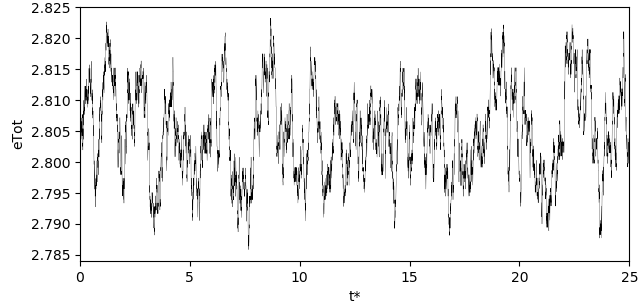
\includegraphics[width=0.7\linewidth]{conservazioneEnergia/eTot0003}}
	\subfigure[{Run $3$, $\Delta t^* = 0.009$}]%\label{fig:libraryvoid}
	{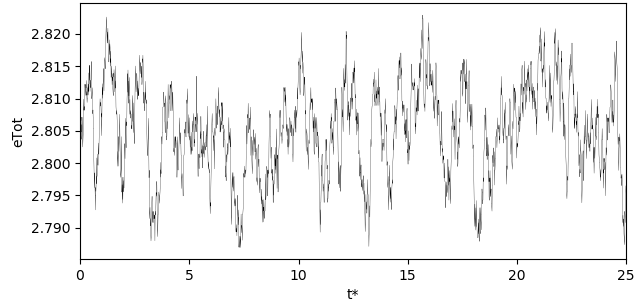
\includegraphics[width=0.7\linewidth]{conservazioneEnergia/eTot0009}}
\end{figure}
\begin{figure}[H]
	\centering 
	\subfigure[{Run $4$, $\Delta t^* = 0.027$}]%\label{fig:board}
	{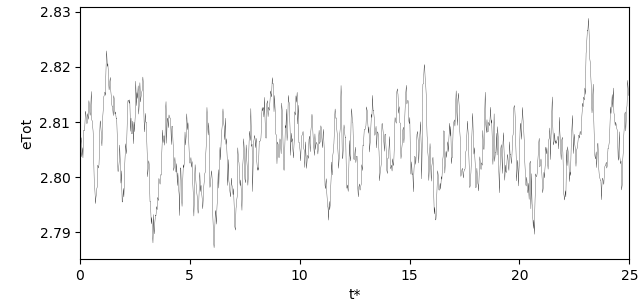
\includegraphics[width=0.7\linewidth]{conservazioneEnergia/eTot0027}}
	\subfigure[{Run $4$, $\Delta t^* = 0.027$}]%\label{fig:board}
	{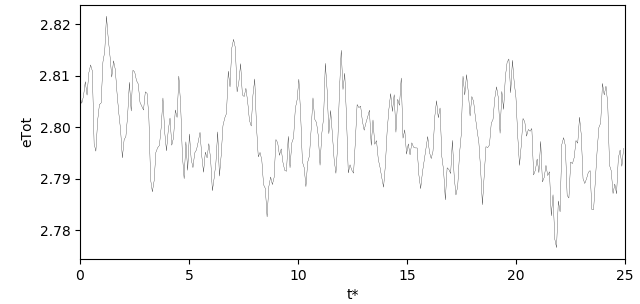
\includegraphics[width=0.7\linewidth]{conservazioneEnergia/eTot0081}}
	\caption{Andamento energia totale}
\end{figure}
\noindent Infatti dall'analisi dei dati otteniamo i seguenti valori per le energie totali medie (per molecola)
\begin{table}[H]
	\centering
	\begin{tabular}{cl} 
		\hline
		$run$	&	$\langle E \rangle /N$ \\
		\hline
		$1$	&	$2.8044$\\
		$2$	&	$2.8049$\\
		$3$	&	$2.8053$\\
		$4$	&	$2.8057$\\
		$5$	&	$2.8020$\\\hline
	\end{tabular}
\end{table}
\medskip
\noindent che confermano la consistenza dell'ipotesi di conservazione dell'energia nelle diverse simulazioni.

\section*{Errori e correlazioni}
Stimiamo ora i valori medi di energia potenziale, pressione e temperatura e calcoliamo i tempi di autocorrelazione e gli errori. Riportiamo i valori ottenuti nella seguente tabella.
\begin{table}[H]
	\centering
	\begin{tabular}{cccccccccc} 
		\hline
		$run$	&	$\langle U  \rangle$	&	$\tau_U$	&	$\sigma_U$ & $\langle P  \rangle$	&	$\tau_P$	&	$\sigma_P$ & $\langle T \rangle$	&	$\tau_T$ & $\sigma_T$ \\
		\hline
		$1$	&	$1.7633$ &	$0.2642$ &	$0.0057$ &	$1.0710$ &	$0.1727$&	$0.00063$&	$0.6941$&	$0.2534$ &	$0.0036$ \\
		$2$	&	$1.7719$ &	$0.2877$ &	$0.0059$ &	$1.0710$ &	$0.1956$&	$0.00071$ &	$0.6886$&	$0.2696$ &	$0.0037$   \\
		$3$	&	$1.7705$ &	$0.2685$ &	$0.0066$ &	$1.0712$ &	$0.2142$&	$0.00078$ &	$0.6898$&	$0.2675$ &	$0.0043$  \\
		$4$	&	$1.7738$ &	$0.2368$ &	$0.0052$ &	$1.0705$ &	$0.1690$&	$0.00067$ &	$0.6879$&	$0.2317$ &	$0.0034$  \\
		$5$	&	$1.7733$ &	$0.2252$ &	$0.0048$ &	$1.0693$ &	$0.2141$&	$0.00078$ &	$0.6858$&	$0.2274$ &	$0.0031$  \\\hline
	\end{tabular}
\end{table}
\medskip

 
\end{document}